\section{Date: 2026-08-07}
\noindent \textbf{Series ID: EXP0008} 

\noindent This series is titled U.S. Exports of Goods by F.A.S. Basis to NICS and has a frequency of Monthly. The units are Millions of Dollars and the seasonal adjustment is Not Seasonally Adjusted.The observation start date is 1985-01-01 and the observation end date is 2012-12-01.The popularity of this series is 1. \\ 

\noindent \textbf{Series ID: A829RE1Q156NBEA} 

\noindent This series is titled Shares of gross domestic product: Government consumption expenditures and gross investment: State and local and has a frequency of Quarterly. The units are Percent and the seasonal adjustment is Not Seasonally Adjusted.The observation start date is 1947-01-01 and the observation end date is 2026-04-01.The popularity of this series is 3. \\ 

\subsection{Raw Regression}
\noindent Regresses the two series against each other directly. A significant result here can come just as easily from both series sharing a long-run trend as from any real relationship.

\begin{center}
\begin{tabular}{lclc}
\toprule
\textbf{Dep. Variable:}       & value\_fred\_A829RE1Q156NBEA & \textbf{  R-squared:         } &     0.417   \\
\textbf{Model:}               &             OLS              & \textbf{  Adj. R-squared:    } &     0.411   \\
\textbf{Method:}              &        Least Squares         & \textbf{  F-statistic:       } &     78.58   \\
\textbf{Date:}                &       Fri, 07 Aug 2026       & \textbf{  Prob (F-statistic):} &  1.55e-14   \\
\textbf{Time:}                &           12:35:32           & \textbf{  Log-Likelihood:    } &   -58.542   \\
\textbf{No. Observations:}    &               112            & \textbf{  AIC:               } &     121.1   \\
\textbf{Df Residuals:}        &               110            & \textbf{  BIC:               } &     126.5   \\
\textbf{Df Model:}            &                 1            & \textbf{                     } &             \\
\textbf{Covariance Type:}     &          nonrobust           & \textbf{                     } &             \\
\bottomrule
\end{tabular}
\begin{tabular}{lcccccc}
                              & \textbf{coef} & \textbf{std err} & \textbf{t} & \textbf{P$> |$t$|$} & \textbf{[0.025} & \textbf{0.975]}  \\
\midrule
\textbf{const}                &      10.8148  &        0.095     &   113.844  &         0.000        &       10.627    &       11.003     \\
\textbf{value\_fred\_EXP0008} &       0.0001  &     1.49e-05     &     8.864  &         0.000        &        0.000    &        0.000     \\
\bottomrule
\end{tabular}
\begin{tabular}{lclc}
\textbf{Omnibus:}       &  7.279 & \textbf{  Durbin-Watson:     } &    0.127  \\
\textbf{Prob(Omnibus):} &  0.026 & \textbf{  Jarque-Bera (JB):  } &    6.829  \\
\textbf{Skew:}          &  0.541 & \textbf{  Prob(JB):          } &   0.0329  \\
\textbf{Kurtosis:}      &  3.540 & \textbf{  Cond. No.          } & 1.56e+04  \\
\bottomrule
\end{tabular}
%\caption{OLS Regression Results}
\end{center}

Notes: \newline
 [1] Standard Errors assume that the covariance matrix of the errors is correctly specified. \newline
 [2] The condition number is large, 1.56e+04. This might indicate that there are \newline
 strong multicollinearity or other numerical problems.

\begin{figure}
\centering
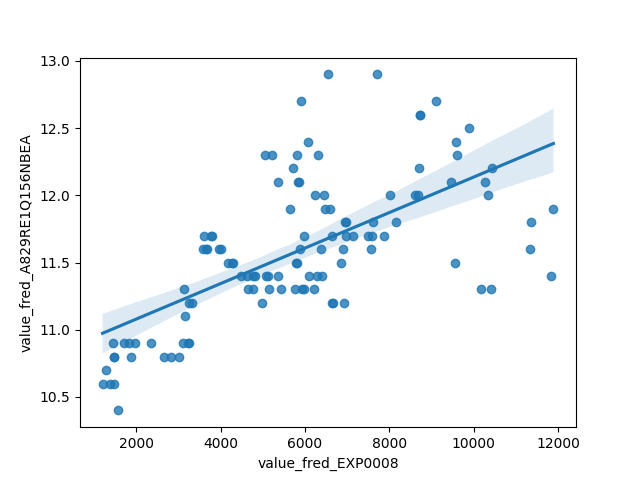
\includegraphics[scale = 0.9]{plots/plot_2026-08-07.png}
\caption{Raw Regression Plot for 2026-08-07}
\end{figure}
\newpage
\subsection{Detrended Regression}
\noindent Regresses the residuals of each series after removing its own linear time trend, so a shared trend can no longer drive the result on its own. A relationship that stays significant here is better evidence of a genuine link between the two series.

\begin{center}
\begin{tabular}{lclc}
\toprule
\textbf{Dep. Variable:}                  & value\_fred\_A829RE1Q156NBEA\_detrended & \textbf{  R-squared:         } &     0.150   \\
\textbf{Model:}                          &                   OLS                   & \textbf{  Adj. R-squared:    } &     0.142   \\
\textbf{Method:}                         &              Least Squares              & \textbf{  F-statistic:       } &     19.42   \\
\textbf{Date:}                           &             Fri, 07 Aug 2026            & \textbf{  Prob (F-statistic):} &  2.45e-05   \\
\textbf{Time:}                           &                 12:35:32                & \textbf{  Log-Likelihood:    } &   -28.396   \\
\textbf{No. Observations:}               &                     112                 & \textbf{  AIC:               } &     60.79   \\
\textbf{Df Residuals:}                   &                     110                 & \textbf{  BIC:               } &     66.23   \\
\textbf{Df Model:}                       &                       1                 & \textbf{                     } &             \\
\textbf{Covariance Type:}                &                nonrobust                & \textbf{                     } &             \\
\bottomrule
\end{tabular}
\begin{tabular}{lcccccc}
                                         & \textbf{coef} & \textbf{std err} & \textbf{t} & \textbf{P$> |$t$|$} & \textbf{[0.025} & \textbf{0.975]}  \\
\midrule
\textbf{const}                           &    5.223e-13  &        0.030     &  1.76e-11  &         1.000        &       -0.059    &        0.059     \\
\textbf{value\_fred\_EXP0008\_detrended} &      -0.0001  &     3.37e-05     &    -4.407  &         0.000        &       -0.000    &    -8.16e-05     \\
\bottomrule
\end{tabular}
\begin{tabular}{lclc}
\textbf{Omnibus:}       &  3.171 & \textbf{  Durbin-Watson:     } &    0.177  \\
\textbf{Prob(Omnibus):} &  0.205 & \textbf{  Jarque-Bera (JB):  } &    2.615  \\
\textbf{Skew:}          & -0.353 & \textbf{  Prob(JB):          } &    0.271  \\
\textbf{Kurtosis:}      &  3.250 & \textbf{  Cond. No.          } &     883.  \\
\bottomrule
\end{tabular}
%\caption{OLS Regression Results}
\end{center}

Notes: \newline
 [1] Standard Errors assume that the covariance matrix of the errors is correctly specified.

\begin{figure}
\centering
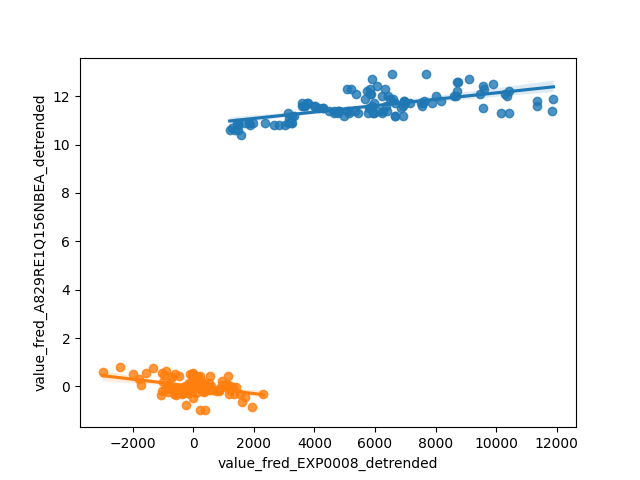
\includegraphics[scale = 0.9]{plots/plot_2026-08-07_detrended.png}
\caption{Detrended Regression Plot for 2026-08-07}
\end{figure}
\newpage
